
\section{Datenbankentscheidungen}
Die Wahl der Datenbank stellt eine essenzielle Entscheidung für das Projekt dar und ist wegweisend dafür, wie Daten gespeichert und verarbeitet werden können. Um die speziellen Anforderungen an Sensora zu erfüllen, beleuchten wir in diesem Kapitel die verschiedenen Datenbankmodelle und kommen abschließend zu einer fundierten Entscheidung.

Grundlegend lassen sich Datenbanken in zwei Hauptkategorien einteilen: SQL-Da\-ten\-ban\-ken und NoSQL-Datenbanken.

SQL-Datenbanken, auch als relationale Datenbanken bezeichnet, basieren auf dem relationalen Datenmodell. Diese Datenbanken sind tabellarisch strukturiert, wobei jede Zeile einen Datensatz bildet und jede Spalte ein spezifisches Feld innerhalb dieses Datensatzes repräsentiert. SQL-Datenbanken sind bekannt für ihre \acs{acid}-Eigenschaften (Atomicity, Consistency, Isolation, Durability), die gewährleisten, dass Transaktionen zuverlässig und sicher ausgeführt werden. Diese Eigenschaften sind besonders wichtig für Anwendungen, bei denen Datenintegrität und Transaktionssicherheit von höchster Bedeutung sind. SQL-Datenbanken erlauben zudem das Setzen von Beziehungen und Verknüpfungen zwischen Datensätzen, was durch integrierte Kontrollmechanismen unterstützt wird. Die Abfragesprache, die in diesen Systemen verwendet wird, ist \ac{sql}. Beispiele für SQL-Datenbanken sind MySQL, PostgreSQL, Oracle Database und Microsoft SQL Server.

NoSQL-Datenbanken hingegen bieten eine breite Palette von Datenbankmodellen, die nicht auf das relationale Modell beschränkt sind. Sie wurden entwickelt, um einige der Einschränkungen von \ac{sql}-Datenbanken zu überwinden und bieten mehr Flexibilität für unterschiedliche Arten von Daten und Anwendungsfällen. Im Gegensatz zu SQL-Datenbanken bieten NoSQL-Datenbanken ein flexibles Datenschema und unterstützen verschiedene Datenmodelle, darunter dokumentenorientierte Modelle, Schlüssel-Wert-Modelle, spaltenorientierte Modelle und graphenbasierte Modelle. Ein weiteres Unterscheidungsmerkmal ist das Prinzip der „eventual consistency“. Dies bedeutet, dass Datenänderungen über die Zeit hinweg konsistent werden, was in verteilten Systemen die hohe Verfügbarkeit gewährleistet, jedoch auch Risiken in Bezug auf Konsistenz und Datenintegrität mit sich bringen kann. Beispiele für NoSQL-Da\-ten\-ban\-ken sind MongoDB, Cassandra, Couchbase, Redis und Neo4j. \cite{Kofler2024}

Aufgrund der Expertise im Entwicklerteam sind MongoDB als objektorientierte Datenbank und PostgreSQL als relationale Datenbank die möglichen Datenbanklösungen für Sensora. Eine Gegenüberstellung beider Technologien führt zur fundierten Auswahl.

\subsection{Exkurs: PostgreSQL}
Um eine fundierte Entscheidung treffen zu können, ist es notwendig, die Architektur und die technischen Hintergründe der PostgreSQL-Datenbank genauer zu betrachten. PostgreSQL, als objektrelationale Datenbank, bietet eine robuste und skalierbare Grundlage für die Speicherung und Verarbeitung von Daten. Im Folgenden wird der Aufbau von PostgreSQL detailliert beschrieben.

\subsubsection{Cluster-Struktur und Prozesse}
Ein PostgreSQL-Server besteht aus einem sogenannten Cluster, der mehrere Datenbanken umfasst. Dieser Cluster kann als die übergeordnete Instanz betrachtet werden, in der alle Datenbanken organisiert sind. Auf einem Server läuft also ein PostgreSQL-Cluster, der die Verwaltung mehrerer Datenbanken übernimmt. Diese Struktur ermöglicht eine effiziente Ressourcennutzung und einfache Skalierung.

\begin{figure}[h]
\centering
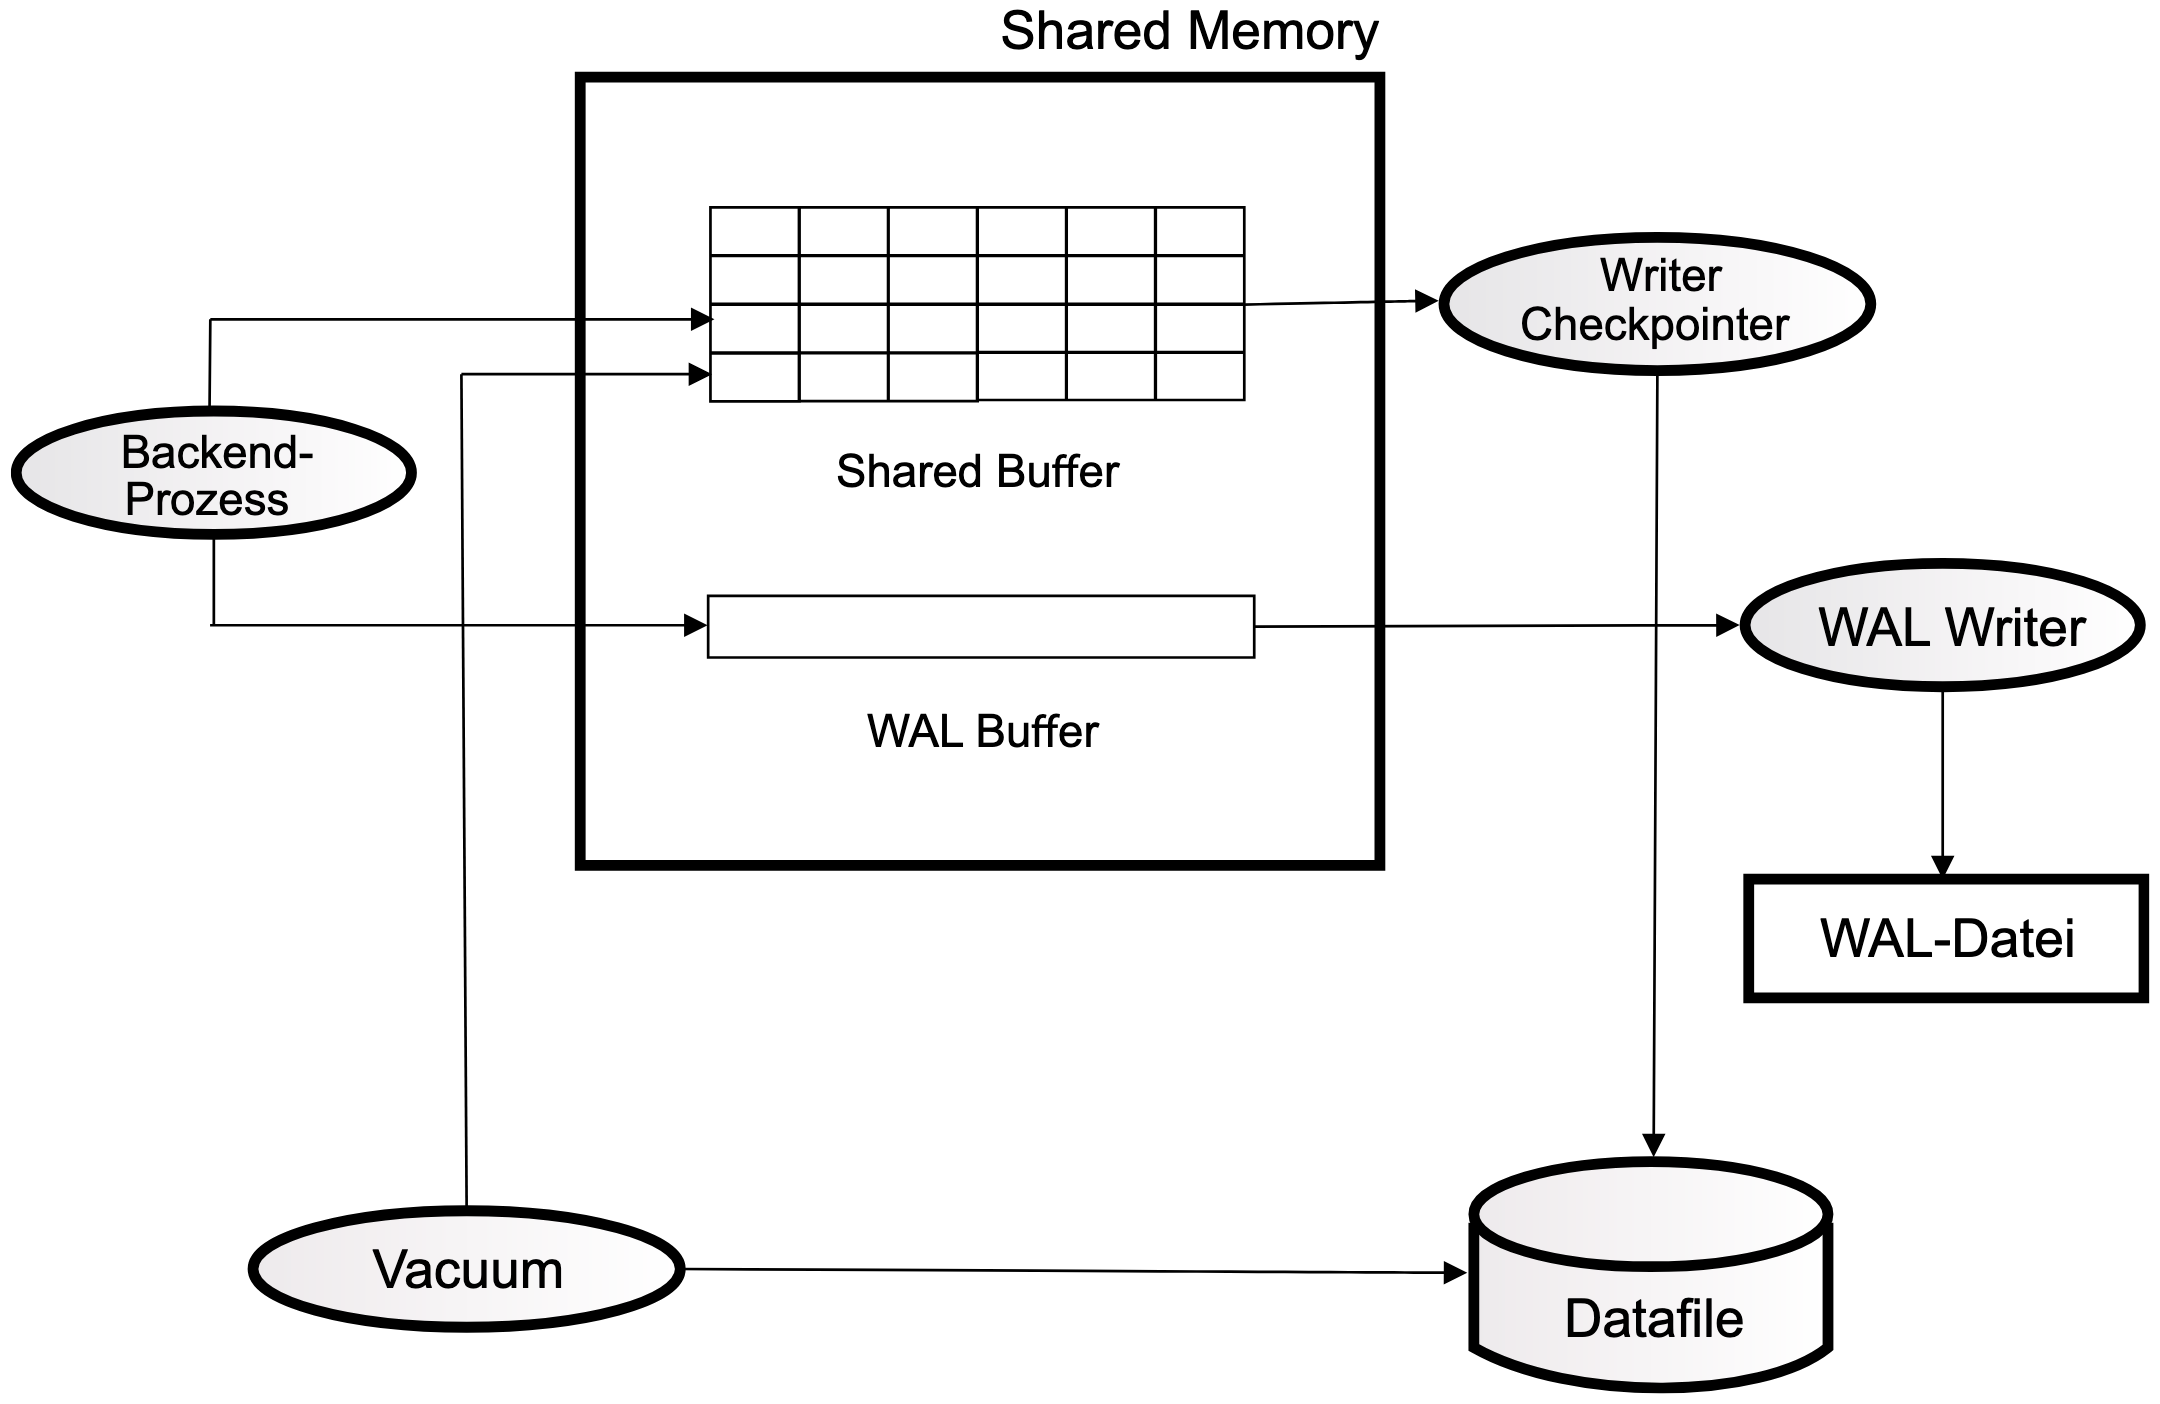
\includegraphics[width=\textwidth]{img/PostgreSQL Aufbau.png}
\caption{PostgreSQL Architektur. Quelle: \cite{Froehlich2022} S. 33 Bild 4.1}
\label{fig:Architektur}
\end{figure}

PostgreSQL besteht aus einer Kombination von Speicher und Prozessen. Bei Unix-Systemen sind diese Prozesse eigenständig, während sie bei Windows als Threads umgesetzt werden. Die wichtigsten Prozesse, die die Funktionalität von PostgreSQL abbilden, sind:
\begin{description}
    \item[Postmaster:] Der Hauptprozess, der die Verwaltung der anderen Prozesse übernimmt.
    \item[Checkpointer:] Dieser Prozess sorgt dafür, dass alle Änderungen in der Datenbank regelmäßig auf die Festplatte geschrieben werden.
    \item[Writer:] Verantwortlich für das Schreiben von geänderten Datenblöcken auf die Festplatte.
    \item[WAL Writer:] Handhabt das Schreiben von Transaktionsdaten in die Write-Ahead Log (WAL).
    \item[Autovacuum Launcher:] Dieser Prozess führt automatische Bereinigungen der Datenbank durch.
    \item[Archiver:] Archiviert die WAL-Dateien für eine verbesserte Rückverfolgbarkeit und Monitoring, besonders wichtig in produktiven Systemen.
    \item[Stats Collector:] Sammelt statistische Daten über die Nutzung von Sessions und Tabellen.
    \item[BGWorker:] Übernimmt verschiedene Hintergrundaufgaben.
\end{description}

\begin{figure}[h]
\centering
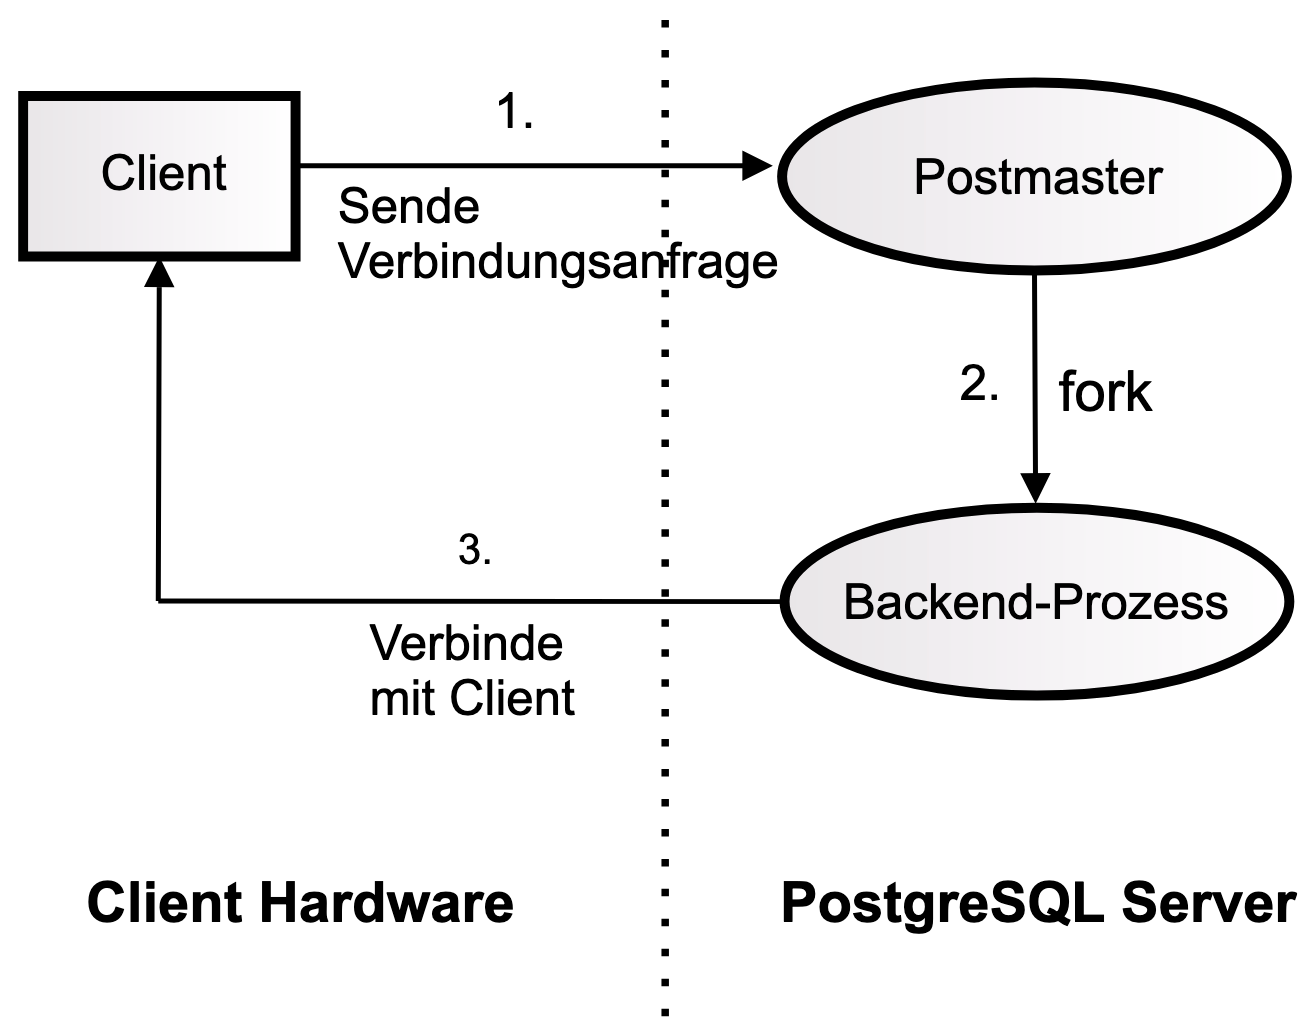
\includegraphics[width=\textwidth]{img/PostgreSQL Verbindungsaufbau.png}
\caption{Verbindungsaufbau von Client zum Server. Quelle: \cite{Froehlich2022} S. 35 Bild 4.3}
\label{fig:Verbindungsaufbau}
\end{figure}

Beim Aufbau einer Verbindung durch einen Client erstellt der Postmaster-Prozess nach erfolgreicher Authentifizierung und Autorisierung einen eigenen Backend-Thread. Die maximale Anzahl gleichzeitig aktiver Backend-Threads ist limitiert (Standard 100), was bedeutet, dass nach Erreichen dieser Grenze weitere Verbindungen abgelehnt werden.

\subsubsection{Speicherverwaltung und Performanceoptimierung}
Die Verwaltung von Speicher und die Optimierung der Zugriffszeiten auf Daten sind entscheidend für die Leistung von PostgreSQL. Da das Lesen von Daten von einer Festplatte vergleichsweise zeitaufwendig ist, setzt PostgreSQL auf verschiedene Mechanismen zur Verbesserung der Performance.

\begin{figure}[h]
\centering
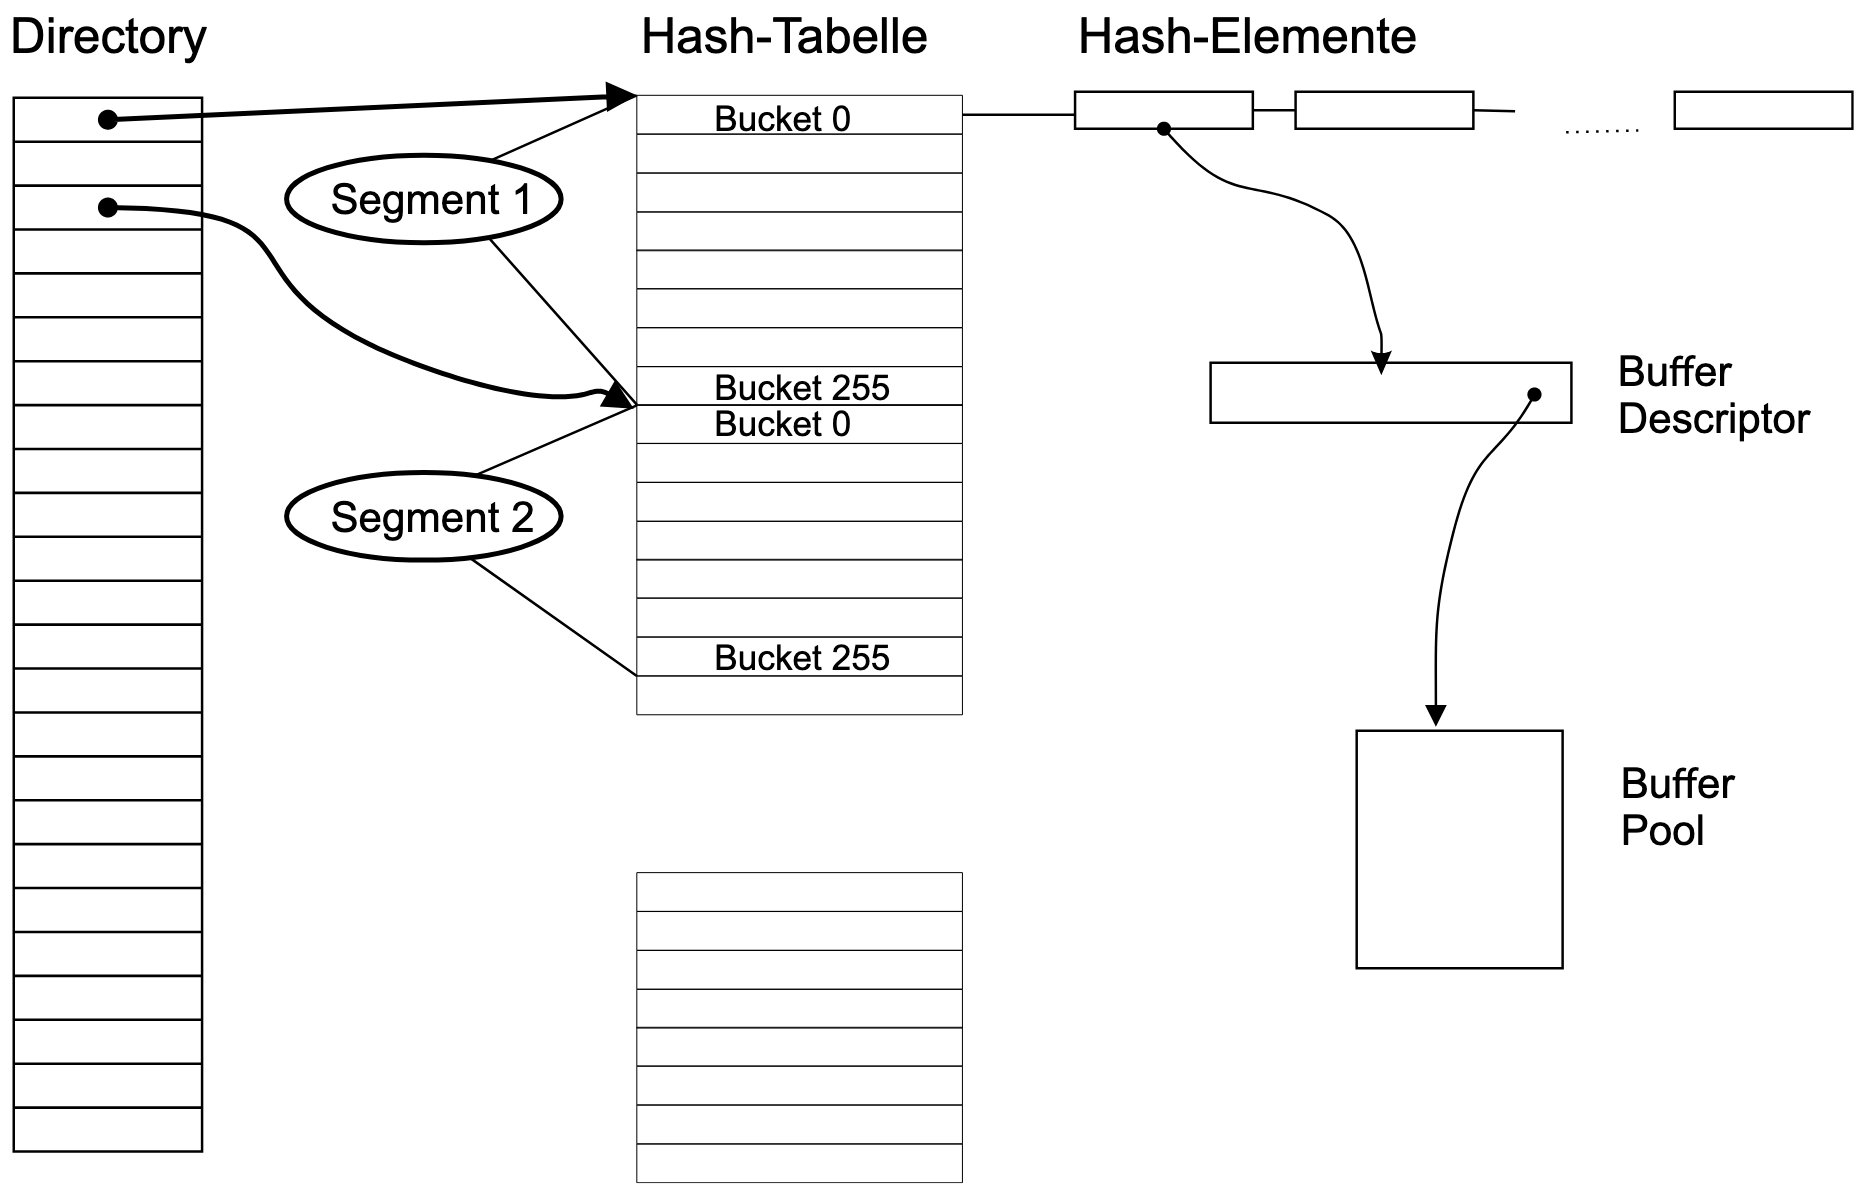
\includegraphics[width=\textwidth]{img/PostgreSQL Speciheraufbau.png}
\caption{PostgreSQL Speicherarchitektur. Quelle:  \cite{Froehlich2022} S. 37 Bild 4.4}
\label{fig:Speicheraufbau}
\end{figure}

\paragraph{Geteilter Speicher (Shared Buffer)}
Der Shared Buffer in PostgreSQL dient dazu, die Anzahl der Operationen auf der Festplatte zu reduzieren, indem er schnellen Speicher im RAM bereitstellt. Er besteht aus einer Hash-Tabelle, Hash-Elementen, einer Bufferbeschreibung und einer Buffersammlung. Die Hash-Tabelle ermöglicht ein schnelles Auffinden von Datensätzen, indem Hashwerte in Segmenten sortiert werden. Diese Segmente können sehr schnell durchsucht werden, da ihre Länge fest ist, was effiziente Speicherzugriffe ermöglicht.

Die Bufferbeschreibung enthält wichtige Steuerungsvariablen, wie z.B. den \code{\url{usage count}}, der die Relevanz eines Datensatzes im Speicher angibt. Der Speicherbereinigungsprozess (Eviction Process) durchsucht regelmäßig den Buffer nach irrelevanten Blöcken. Blöcke, die als irrelevant eingestuft werden, können überschrieben werden, sobald neuer Speicherplatz benötigt wird.

\paragraph{WAL Buffer und Checkpoints}
Der \ac{wal} Buffer ist darauf ausgelegt, Daten effizient auf die Festplatte zu schreiben. Dadurch müssen schreibende Prozesse nicht auf die tatsächliche Schreiboperation warten, sondern können die zu schreibenden Daten in den Buffer verlagern. Der \ac{wal} Buffer wird in regelmäßigen Intervallen (Standard 200 Millisekunden) überprüft und die Daten werden im Permanentspeicher gesichert, um die Ausfallsicherheit zu gewährleisten.

\code{Insert}-, \code{Update}- und \code{Delete}-Anweisungen werden über den \ac{wal}-Buffer verarbeitet. Diese Anweisungen werden in sogenannten \ac{wal}-Records gespeichert und sichern den Zustand der Daten auch bei einem Systemausfall. Ein Checkpoint, der den Speicherinhalt endgültig auf die Festplatte schreibt, wird unter bestimmten Bedingungen ausgeführt, wie etwa nach Ablauf eines festgelegten Intervalls, Erreichen einer bestimmten Buffergröße oder dem manuellen Auslösen eines Checkpoints.

\paragraph{Mehrere Datenblockversionen und Defragmentierung}

PostgreSQL unterstützt die gleichzeitige Bearbeitung von Datensätzen durch mehrere Sessions. Um sicherzustellen, dass sich die Sessions nicht gegenseitig beeinträchtigen, erhalten Datensätze eine Versionsnummer. Diese ermöglicht es, bei gleichzeitigen Abfragen und Bearbeitungen konsistente Daten bereitzustellen. Wenn eine Abfrage gestartet wird, kann anhand der Versionsnummer bestimmt werden, welcher Datensatz zum Zeitpunkt des Abfragestarts aktuell war.

Alte Datensätze, die nicht mehr benötigt werden, werden gelöscht, wodurch Lücken in der Tabelle entstehen. Diese Lücken werden durch den Autovacuum-Prozess freigegeben, sodass der Speicher für neue Datenblöcke verwendet werden kann. Bei Bedarf führt PostgreSQL ein \code{fullvacuum} durch, der die Tabelle vollständig defragmentiert, um Speicherplatz zurückzugewinnen und die Integrität der Versionsnummern zu gewährleisten.

\subsubsection{Permanentspeicherverwaltung}

Die Datenbanken von PostgreSQL werden im Verzeichnis \code{base} gespeichert, während der Tablespace in einem separaten Verzeichnis liegt. Tabellen und Indizes werden in Dateien von maximal einem Gigabyte Größe gespeichert; bei Überschreiten dieser Größe wird eine weitere Datei angelegt. Zusätzlich werden Dateien mit den Endungen \code{\_fsm} (Free Space Map) zur Adressierung des freien Speicherplatzes und \code{\_vm} (Visibility Map) zur Markierung von veralteten Datensätzen gepflegt.

Die Datenblocksammlung (Page) enthält Pointers auf die tatsächlichen Datenblöcke (Tuples). Jeder Datenblock wird durch eine Kombination aus der Datenblocksammlungsnummer und dem Offset des Pointers identifiziert. \cite{Froehlich2022}

\subsection{Exkurs: MongoDB}
MongoDB ist eine führende dokumentenorientierte NoSQL-Datenbank, die sich durch ihre Flexibilität und Skalierbarkeit auszeichnet. Sie wurde entwickelt, um einige der Einschränkungen traditioneller relationaler Datenbanken zu überwinden und bietet eine leistungsfähige Lösung für Anwendungen, die große Mengen an unstrukturierten oder semi-strukturierten Daten verarbeiten müssen. Im Gegensatz zu relationalen Datenbanken, die auf einem festen Schema basieren, erlaubt MongoDB ein dynamisches, schemaloses Datenmodell, das sich ideal für moderne, agile Entwicklungsprozesse eignet. In diesem Exkurs werden die Architektur und die technischen Merkmale von MongoDB detailliert beleuchtet, um deren Eignung für das \ac{nomtis}-Projekt zu bewerten.

\subsubsection{Speicherstruktur und Organisation}
MongoDB speichert Daten im \ac{bson}-Format, einem binären Format, das speziell für die Speicherung von Dokumenten mit \ac{json}-Syntax entwickelt wurde. \ac{bson} bietet eine effiziente Speicherung und Verarbeitung von Dokumenten, da es im Vergleich zu herkömmlichem \ac{json} kompakter und schneller zu verarbeiten ist. \ac{bson}-Dokumente können direkt in \ac{json} konvertiert werden, was die Integration mit Anwendungen erleichtert, die \ac{json} verwenden.

Die Speicherorganisation in MongoDB ist hierarchisch aufgebaut:
\begin{description}
    \item[Datenbank:] An der Spitze steht eine Datenbank, die mehrere Sammlungen (engl. Collections) enthalten kann.
    \item [Katalog:] Darunter befindet sich der Katalog, der Informationen über die Sammlungen und Indizes speichert.
    \item [Sammlung (engl. Collection)]: Eine Sammlung ist eine Gruppe von Dokumenten, die thematisch zusammengehören und ähnliche Strukturmerkmale aufweisen.
    \item [Dokument:] Auf der untersten Ebene steht das Dokument, das die eigentlichen Daten enthält.
\end{description}

\subsubsection{Katalog und Speicherverwaltung}

Der Katalog von MongoDB ist für die Verwaltung der Metadaten von Sammlungen und Indizes verantwortlich. Es gibt zwei Arten von Katalogen:
\begin{description}
    \item[Persistenter Katalog:] Dieser speichert Informationen dauerhaft auf der Festplatte und stellt sicher, dass Metadaten auch nach einem Neustart des Systems verfügbar bleiben. Der persistente Katalog wird in BSON-Dateien mit der Endung \code{\_mdb\_catalog} gespeichert und enthält Details über die Eigenschaften und Indizes der Sammlungen.
    \item [Memory-Katalog:] Der Memory-Katalog hält die Metadaten im RAM vor, um schnellen Zugriff zu gewährleisten und Ladezeiten zu minimieren. Operationen wie das Erstellen, Suchen, Iterieren und Schließen von Sammlungen werden im Memory-Katalog durchgeführt.
\end{description}

Um Dateninkonsistenzen zu vermeiden, wird der Memory-Katalog regelmäßig mit dem persistenten Katalog synchronisiert. Eine Versionsverwaltung stellt sicher, dass Änderungen korrekt nachvollzogen werden können, ohne dass es zu Lese-Schreib-Kollisionen kommt. MongoDB verwendet dabei das Copy-on-Write-Prinzip, bei dem nur dann eine Kopie des Datensatzes erstellt wird, wenn tatsächlich Änderungen vorgenommen werden. Dies minimiert den Speicherbedarf und erhöht die Effizienz.

\subsubsection{Speicherverwaltung und Defragmentierung}
Beim Löschen eines Eintrags in MongoDB erfolgt dieser Prozess in zwei Schritten:
\begin{enumerate}
    \item Löschen des Katalogeintrags: Zunächst wird der Eintrag sowohl im Memory-Katalog als auch im persistenten Katalog entfernt. Ein Verweis auf die Sammlung wird an den sogenannten \glqq Reaper\grqq{} übergeben, um sicherzustellen, dass keine neuen Zugriffe auf die Sammlung erfolgen, während aktive Lesezugriffe abgeschlossen werden.
    \item Endgültiges Löschen: Nachdem sichergestellt wurde, dass kein Rollback erfolgen kann, der die Daten der Sammlung wiederherstellen könnte, werden die Daten endgültig gelöscht.
\end{enumerate}

Freier Speicher, der durch das Löschen von Daten entsteht, wird in regelmäßigen Abständen für neue Datensätze freigegeben. Wenn der Speicher fragmentiert wird und viele kleine Lücken entstehen, führt MongoDB eine Defragmentierung durch. Dieser Prozess ordnet den Speicher neu an, kann jedoch Lese- und Schreiboperationen blockieren, was die Performance beeinträchtigen könnte. Daher sollte die Defragmentierung möglichst selten durchgeführt werden.

\subsubsection{Indizes und Abfragen}
Indizes in MongoDB werden hauptsächlich als B-Baum-Strukturen gespeichert, die eine effiziente Suche und Sortierung von Daten ermöglichen. Ein B-Baum-Index speichert die Daten strukturiert, ähnlich wie ein Dokument, und ermöglicht schnelle Zugriffe auf häufig abgefragte Felder. MongoDB erlaubt es auch, benutzerdefinierte Speicherstrukturen für Indizes zu erstellen, um spezifische Anwendungsanforderungen zu erfüllen. \cite{IamXander2024} \cite{themattman2024}

\subsubsection{BSON - Binary JSON}

\ac{bson} ist das zugrunde liegende Format für die Speicherung von Dokumenten in MongoDB. Es handelt sich dabei um ein binäres Format, das sogenannte Key-Value-Paare speichert und direkt in \ac{json} konvertiert werden kann. \ac{bson} ist jedoch deterministischer als \ac{json}, da es keine Flexibilität in der Darstellungsform bietet. Dies bedeutet, dass ein Datensatz in \ac{bson} immer in einer einzigen, festen Form dargestellt wird.

Ein \ac{bson}-Dokument beginnt immer mit einem 32-Bit-Ganzzahlwert, der die Länge des Dokuments angibt, und endet mit einem Null-Byte. Aufgrund dieser Struktur kann ein \ac{bson}-Dokument maximal ca. 2,147 Gigabyte an Daten umfassen. Die verschiedenen Datentypen, die \ac{bson} unterstützt, umfassen unter anderem:
\begin{description}
    \item[Int32 und Int64:] 4- bzw. 8-Byte lange Ganzzahlen.
    \item[Double:] 8-Byte lange Gleitkommazahlen nach dem IEEE 754-Standard.
    \item[Decimal128:] 16-Byte lange Gleitkommazahlen für hohe Präzision.
    \item[Array:] Ein Feld, das eine Liste von Werten speichert, wobei die Elemente wie Dokumente behandelt werden.
    \item[Null-Wert:] Ein spezieller Marker, der das Fehlen eines Wertes kennzeichnet.
    \item[Min- und Max-Schlüssel:] Marker, die den minimalen bzw. maximalen Wert eines Feldes darstellen.
\end{description}

Die strikte Struktur von \ac{bson} sorgt für eine konsistente und effiziente Speicherung und Verarbeitung von Dokumenten, was MongoDB zu einer leistungsfähigen Lösung für Anwendungen macht, die flexible und skalierbare Datenbanken benötigen. \cite{Velikhov}

\subsection{Diskurs: Vergleich von PostgreSQL und MongoDB für NOMTIS}
Die Auswahl der geeigneten Datenbanklösung ist ein zentraler Aspekt bei der Entwicklung von \ac{nomtis}. Da die internen Richtlinien PostgreSQL und MongoDB als verfügbare Optionen vorsehen, ist es entscheidend, die spezifischen Anforderungen von \ac{nomtis} zu analysieren und zu bestimmen, welche der beiden Datenbanken diese am besten erfüllt.

\subsubsection{Technische Anforderungen an NOMTIS}
\ac{nomtis} muss Benachrichtigungen effizient speichern, verwalten und flexibel verarbeiten können. Ein Hauptmerkmal von \ac{nomtis} ist die Fähigkeit, Benachrichtigungen mit potenziell komplexen und verschachtelten Datenstrukturen zu verwalten. Diese Datenstrukturen können variieren und sind oft nicht im Voraus vollständig definiert. Zudem sind eine hohe Zuverlässigkeit, Konsistenz und Skalierbarkeit erforderlich, um den Anforderungen eines modernen Benachrichtigungssystems gerecht zu werden.

\subsubsection{PostgreSQL: Technische Stärken und Grenzen}
PostgreSQL ist eine relationale Datenbank, die für ihre starke Unterstützung von \ac{acid}-Transaktionen, Datenintegrität und komplexen relationalen Abfragen bekannt ist. Diese Eigenschaften machen PostgreSQL ideal für Anwendungen, bei denen strenge Konsistenzanforderungen und komplexe Datenbeziehungen im Vordergrund stehen.

Die feste Struktur von PostgreSQL kann jedoch zu Einschränkungen führen, wenn es darum geht, dynamische und verschachtelte Datenstrukturen zu verwalten. Änderungen am Datenmodell erfordern eine Anpassung des Schemas, was in einem dynamischen Umfeld, wie es \ac{nomtis} erfordert, potenziell problematisch sein kann. Zudem ist PostgreSQL weniger effizient im Umgang mit tief verschachtelten oder unvorhersehbaren Datenstrukturen, was die Flexibilität des Systems einschränken könnte.

\subsubsection{MongoDB: Flexibilität und Skalierbarkeit}
MongoDB hingegen ist eine dokumentenorientierte NoSQL-Datenbank, die sich durch ihre schemalose Architektur und hohe Flexibilität auszeichnet. Die Speicherung erfolgt im BSON-Format, das eine effiziente Handhabung von \ac{json}-ähnlichen Dokumenten ermöglicht. Diese Struktur erlaubt es, Daten ohne festes Schema zu speichern, was für \ac{nomtis} von Vorteil ist, da die Benachrichtigungen beliebig komplexe und verschachtelte Daten enthalten können.

Ein weiterer zentraler Vorteil von MongoDB ist seine horizontale Skalierbarkeit. MongoDB unterstützt das sogenannte \glqq Sharding \grqq, bei dem Daten über mehrere Server verteilt werden, um eine hohe Verfügbarkeit und Performance sicherzustellen. Diese Fähigkeit zur horizontalen Skalierung ist besonders in einer Umgebung wie der \ac{sit} von Bedeutung, wo das Datenvolumen und die Anzahl der Nutzer kontinuierlich wachsen können.

Laut einer Untersuchung der MongoDB-Datenbank von Anjali Chauhan bietet MongoDB darüber hinaus eine hohe Leistung durch die Verwendung eingebetteter Datenmodelle, die E/A-Aktivitäten reduzieren, sowie durch Indizes, die schnellere Abfragen ermöglichen. \cite{Chauhan2019}
Diese Leistungsmerkmale machen MongoDB besonders geeignet für Anwendungen, die auf hohe Geschwindigkeit und effizienten Datenzugriff angewiesen sind.

\subsubsection{Schlussfolgerung: PostgreSQL als geeignete Wahl für Sensora}
Im Projekt Sensora ergibt sich aus den strukturellen Anforderungen und den funktionalen Zugriffsmustern ein klarer Bedarf an einem relationalen, transaktional konsistenten Datenbanksystem. Die Datenstruktur ist vordefiniert und weitgehend stabil. Pflanzen, Sensoren, Aktoren, Gruppen und Räume bilden klar abgegrenzte Entitäten mit definierten Beziehungen zueinander. Diese Relationen sind nicht nur logisch konzipiert, sondern stellen funktionale Notwendigkeiten dar – etwa wenn Sensoren bestimmten Pflanzen zugeordnet sind oder Aktionen nur innerhalb definierter Gruppenzugehörigkeiten zulässig sind.

Die Abfrageanforderungen im operativen Betrieb bestehen aus einer Mischung aus punktuellen Zugriffen (etwa auf aktuelle Sensorwerte oder Soll-Ist-Vergleiche) und zeitbasierten Auswertungen über große Datenmengen – insbesondere für die letzten 24 Stunden. Diese Anforderungen sind auf ein konsistentes, indexoptimiertes Schema angewiesen, das Joins effizient unterstützt und sich nicht durch Schema-Flexibilität, sondern durch strukturelle Integrität auszeichnet. Gleichzeitig ist paralleler Zugriff durch mehrere Microservices erforderlich, sodass Transaktionssicherheit und Isolation nicht nur erwünscht, sondern notwendig sind, um Inkonsistenzen bei konkurrierenden Schreiboperationen zu vermeiden.

PostgreSQL bietet genau für diese Art von Workload die passende Grundlage. Die stark normierten Strukturen des Sensora-Datenmodells profitieren von PostgreSQLs ausgefeilter Optimierung relationaler Abfragen, der zuverlässigen Durchsetzung referenzieller Integrität sowie der Möglichkeit, durch gezieltes Indexing auf Zeitstempel-Feldern hochfrequente historische Abfragen performant abzubilden. Selbst bei wachsendem Datenvolumen lassen sich durch Partitionierung oder die spätere Ergänzung durch TimescaleDB – ohne Verlassen der PostgreSQL-Basis – die Performanceanforderungen langfristig erfüllen, ohne strukturelle Kompromisse einzugehen.

Die fehlende Notwendigkeit für dynamische Schemas, polymorphe Dokumente oder eingebettete Strukturen eliminiert die Hauptargumente für ein dokumentenbasiertes System wie MongoDB. Vielmehr würde dessen Flexibilität in diesem Kontext eher potenzielle Inkonsistenzen begünstigen und zusätzliche Validierungslogik auf Anwendungsebene erforderlich machen – ein Mehraufwand, der durch das klar strukturierte Datenmodell nicht gerechtfertigt ist.

In Summe ist PostgreSQL damit nicht nur die technisch bessere Wahl, sondern die natürlichere Fortsetzung der bereits im Projektdesign angelegten Prinzipien: strukturierte, konsistente und integrierte Datenhaltung, auf die performant und sicher gleichzeitig von vielen Systemkomponenten zugegriffen werden kann.
